\chapter{Algorithm Implementation}
In this chapter some of the algorithm in the theory chapter are combined, tested and evaluated. The goal is to find the most robust combination of algorithms to detect the pupil even in a very demanding data set like the LPW. The LPW data set is already discussed in its chapter and will not be discussed here again. In general the evaluation can be split up into two part. The first part is localization of the pupil and second part is finding the pupil ellipse. The importance of the localization is that with the information of the location of the pupil it is possible to create a region of interest (ROI). This has the benefit that in the second part the image size is already decreased and additional noise can be even more limited. Also the computational effort is reduced because the image size is smaller. Important to note is, that all algorithms make the basic assumption, that the pupil is always visible. So blinking is not counted as a failure and excluded of the evaluation if possible. For detecting blinking, other algorithms need to be used to preprocess every frame and detect if the eye is closed or not. 


\section{Localization}
For the localization mainly thresholding, edge detection and haar-like features were implemented and can now be evaluated. To make thresholding more flexible a semi adaptive algorithm was created to choose the best fitting threshold value. The histogram is used to determine the highest peak in the low intensity range. This value is then used to threshold the image. 
\begin{equation}
    t = \text{argmax} \{h(i) | i \in [0,255]\}
\end{equation}
With $h(i)$ being the histogram of the image. The threshold value is then used to calculate a range for using double thresholding to extract the pupil. The image is modified by setting all values below and above the threshold value to 0. 
\begin{equation}
    f(x,y)= \begin{cases}
        0 &iff \quad I(x,y) < t-35 \quad \text{or} \quad I(x,y) > t+25 \\
        I(x,y) &otherwise
    \end{cases}
\end{equation}
\subsection{Thresholding}
Whereas the under limit of the threshold is set lower than the higher limit. This derives from testing and can be concluded, that the probability that the pixels with lower intensity values belongs to the pupil is higher than the probability that the pixels with higher intensity values belong to the pupil. In a environment with almost no noise and most important no reflections this approach works very well. But as also already mentioned in the theory section, reflections lead to a less higher peak in the histogram and the possibility exist that the threshold value has no peak in the lower values range and therefore leads to a faulty result that can not be used to create an ROI or use it with edge detection to find the boundary of the pupil. Also it is important to note that with this thresholding approach the mask created is not a binary mask but a mask with values between $[t-35, t+25]$. But the possibility to use the binary mask still exist and the all contours found in this threshold range are evaluated by their circularity and similarity to an ellipse. The best fitting contour is then used to create the ROI or ellipse fit directly to find the ellipse parameters. 
[RESULTS]
This method works in a environment with almost no noise flawless, it is has benefit to reach the goal in almost realtime but in with the LPW data set it is keen to strugle with most of the conditions and is therefore not usefull for the LPW data set.

\subsection{Edge detection}
Edge detection is strongly effected by noise and therefore the preprocessing is key for useful results. Every frame undergoes the same preprocessing as in the other algorithms but a gaussian blur is used additionally to smooth fast changing intensity regions out.  Even though the gaussian blur is used, there is still information missing that is covered by noise. The edges are detected but the same problem as with thresholding arises here. By using Sobel and than the Canny edge detection the results are useful in a environment with almost no noise but as already said, LPW is known for its noise and reflections. Canny edge detection needs two threshold parameters to work properly and also here arises the problem that these parameters need to be adaptive to the environment which can be tricky. 
[RESULTS]

\subsection{Haar-like features}
The Haar-like feature is the approach that is proposed by this thesis to find the region of interest. It has the best detection rate of all approaches tested on the LPW data set and is therefore the best approach to find the ROI. The Haar-like feature is constructed as described in the theory part and is shown in \ref{fig:haar_pupil}. 
The calculation of the feature vector is done by using the integral image and is done 3 times with variating Radius $r$ all feature vectors are then compared and the location of the highest response is returned as a point that lies on the pupil. 

\begin{figure}[h]
    \centering
    \begin{subfigure}{0.5\textwidth}
        \centering
        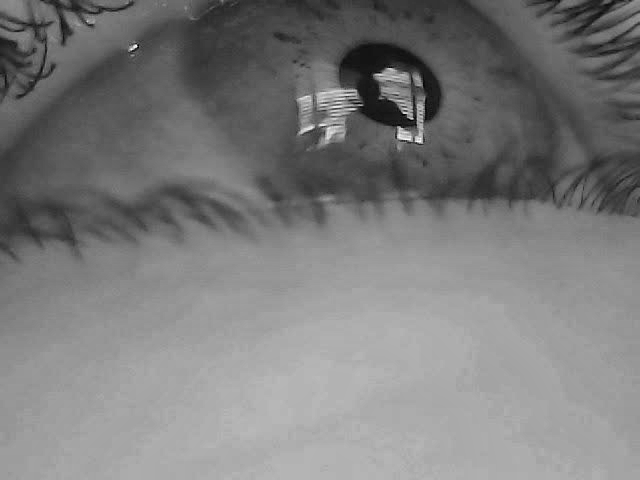
\includegraphics[width=0.9\linewidth]{plots/results/originalbest.png}
        \caption{Original Frame}
    \end{subfigure}%
    \hfill
    \begin{subfigure}{0.5\textwidth}
        \centering
        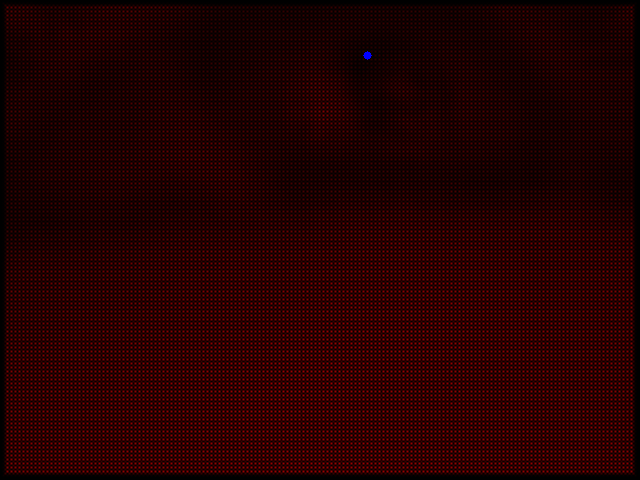
\includegraphics[width=0.9\linewidth]{plots/results/responsehaarbest.png}
        \caption{feature vector, blue is the best response}
    \end{subfigure}%
 
    \caption{Feature vector for pupil detection}
    \label{fig:limit_haar}
\end{figure}

The stronges response lies then within the pupil and the location is then used to create a ROI. In this case a ROI of $110 x 110$ was the norm but depending on the rescaling of the frames this can be adapted. Important to note is, that the returned point in the pupil is not given to be in the center. This in an important fact when choosing the size of the ROI that is created. 
But this approach is still not perfect and even though it can handle noise really good, there are limits to the amount of noise until the algorithm fails. Also the algorithm is not able to detect the pupil when the eye is closed.

\begin{figure}[h]
    \centering
    \begin{subfigure}{0.5\textwidth}
        \centering
        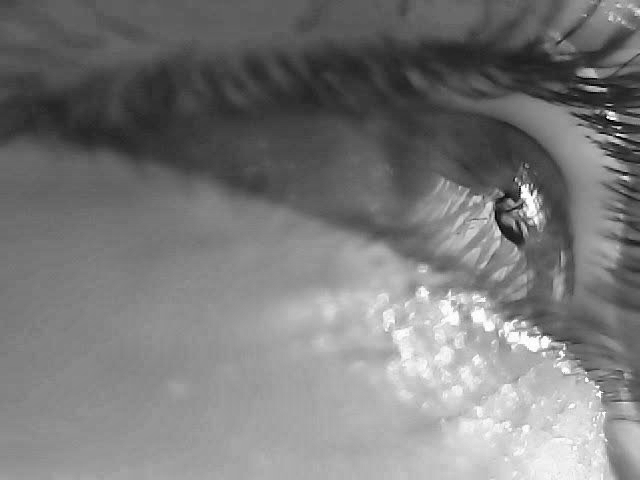
\includegraphics[width=0.9\linewidth]{plots/results/originalworst.png}
        \caption{Extreme noise example}
    \end{subfigure}%
    \hfill
    \begin{subfigure}{0.5\textwidth}
        \centering
        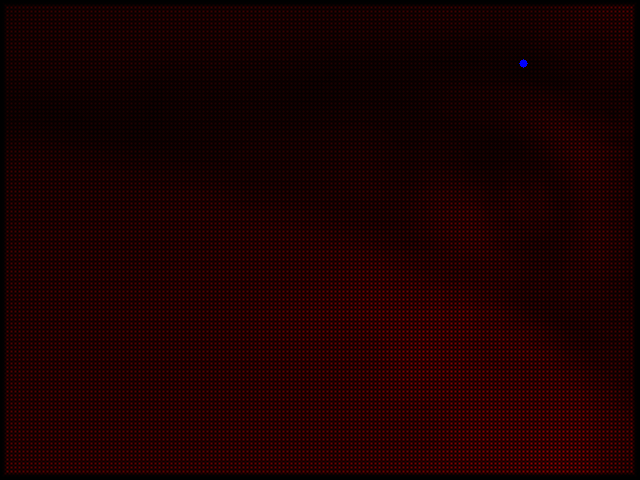
\includegraphics[width=0.9\linewidth]{plots/results/responsehaarworst.png}
        \caption{feature vector result with best response}
    \end{subfigure}%
 
    \caption{Limits to the Haar-like feature approach}
    \label{fig:limit_haar}
\end{figure}
The problem with the LPW data set is, that it is so versatile and the conditions change during the recording. This makes it hard to find an approach that can adapt to all the conditions and still perform well in a given time interval. The implementation can still be improved and sped up, in the Haar-like feature the following libraries were used to speed up the algorithm: 

\begin{python}
from concurrent.futures import ThreadPoolExecutor
from numba import njit
    \end{python}
ThreadPool Executor makes it possible to use multithreading and njit compiles the sliding window over the integral image of the Haar-like feature to machine code for more efficient calculation.

\section{Ellipse parameter estimation}
In the second part of an pupil detection algorithm it is necessary to make use of the informations from the first part and build on this foundation and find the five ellipse parameter: center: $(x,y)$, axis: (major, minor) and angle. The LPW has labels for the center only of the pupil and therefore only the center can be used to evaluate the performance of the algorithms. A second evaluation has to be done manually by inspecting the fit of the ellipse to the pupil. This is hard to evaluate with numerical methods and the result needs therefore to be taken with a grain of salt. In this section 4 different algorithms will be discussed and evaluated: The OpenCV ellipse fit based on contours (binary thresholding), ACWE with OpenCV Ellipse fit, ACWE combined with RANSAC, and Canny edge detection with OpenCV Ellipse fit. 

\subsection{Thresholding and OpenCV ellipse fit}
The benefit of this method is that it can almost run in realtime and still perform well in certain frames where the noise is low and the pupil is clearly visible. But as already mentioned in the localization part, this method is not robust enough to handle the LPW data set. The thresholding is done with the same approach as in the localization part and the binary mask is then used to find the contours. The contours are then evaluated by their circularity and similarity to an ellipse. The best fitting contour is then used to fit an ellipse with the OpenCV ellipse fit function. The OpenCV ellipse fit function is based on the least square method and therefore very robust and fast. The ellipse fit is then evaluated by the center and the distance to the ground truth center. The problem with least square method is, lies in the definition itself. Because the method tries to find an ellipse that minimizes the distance from every point on the boundary of the binary mask to the ellipse curve. When the pupil is partially covered by noise, the contour does not match the original shape of the pupil and does not represent the total pupil boundary. Using least square method in this case leads to a faulty ellipse fit where the result is not usable. The amount of outliers is to high and the ellipse fit is not accurate enough because there is information missing. 
\begin{figure}[h]
    \centering
    \begin{subfigure}{0.3\textwidth}
        \centering
        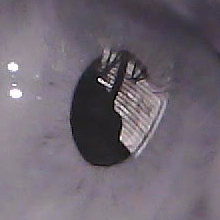
\includegraphics[width=0.9\linewidth]{plots/results/roi_text_resutls.png}
        \caption{ROI}
    \end{subfigure}%
    \hfill
    \begin{subfigure}{0.3\textwidth}
        \centering
        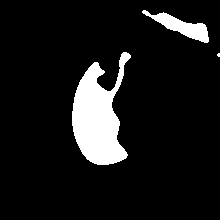
\includegraphics[width=0.9\linewidth]{plots/results/roi_binary_ellipse.png}
        \caption{Binary thresholding}
    \end{subfigure}%
    \hfill
    \begin{subfigure}{0.3\textwidth}
        \centering
        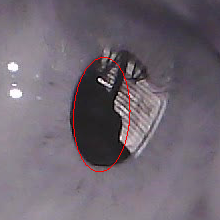
\includegraphics[width=0.9\linewidth]{plots/results/roi_result_binary_ellipse.png}
        \caption{OpenCV Ellipse fit}
    \end{subfigure}%
    \caption{Binary thresholding with OpenCV ellipse fit}
    \label{fig:binary_threshold_ellipse_fit}
\end{figure}

\subsection{Canny edge detection with OpenCV ellipse fit}


\subsection{ACWE with OpenCV ellipse fit}


\subsection{ACWE combined with RANSAC}

